\documentclass[11pt]{article}
\usepackage[a4paper,margin=2.5cm]{geometry}
\usepackage[T1]{fontenc}
\usepackage{booktabs}
\usepackage{graphicx}
\usepackage{xurl}
\usepackage[hidelinks]{hyperref}
\hypersetup{pdftitle={Marking the Note Is Not Enough: Datamarking, Roman Urdu and Argument Checks Against Hidden Instructions for Small Local Tool Agents},pdfauthor={Muzammal Hussain}}
\usepackage{natbib}

\title{Marking the Note Is Not Enough:\\Datamarking, Roman Urdu and Argument Checks\\Against Hidden Instructions for Small Local Tool Agents}
\author{Muzammal Hussain\\
\small Independent researcher, Glasgow, United Kingdom\\
\small \href{mailto:muzammal@masmatixinnovations.co.uk}{muzammal@masmatixinnovations.co.uk}\\
\small ORCID: \href{https://orcid.org/0009-0001-2570-5686}{0009-0001-2570-5686}}
\date{\small November 2026}

\begin{document}
\maketitle

\begin{abstract}
A clinic that runs a small language model locally as a tool-using assistant will pass it patient notes that it did not write, in English and in code-mixed Roman Urdu. A note can carry a hidden instruction. We built 40 invented physiotherapy-clinic tasks, each in English and Roman Urdu, with one hidden instruction per task: either an action outside the task (send the record to an outside address, delete it) or an allowed action with the wrong argument (the right booking under another patient's ID, an approved referral sent to another address). Four local models (Llama 3.1 8B, Mistral 7B, Qwen2.5 3B and 7B) proposed tool calls at temperature 0 with a plain prompt and with \emph{datamarking}, a prompt defence that interleaves the untrusted note with a marker character. With the plain prompt the models followed the hidden instruction in 47.5--72.5\% of tasks. Pooled over models, datamarking cut this from 83 to 40 of 160 model--task pairs in English and from 97 to 56 in Roman Urdu (task-level permutation tests, both $p<0.0001$), but the effect depended on the model: from 20 to 2 of 40 for Llama in English, and from 19 to 16 (not significant) for Qwen2.5 7B. Datamarking almost removed out-of-scope attacks in English (29 to 2 of 80) but not in Roman Urdu (45 to 26; 2 vs 26 after datamarking, $p=0.0005$); over all attacks the language gap after datamarking was smaller and not significant (40 vs 56, $p=0.089$). The larger Qwen was not safer than the smaller one. A permission rule on action names let through every wrong-argument attack that a model followed (174 of 640 attacked replies), while checking each call's patient, recipient and date against the staff request let none through and blocked no correct action. For small local agents, a prompt-level marker is a useful extra layer but not a control; the control is an argument check in code, bound to the trusted request.
\end{abstract}

\section{Introduction}
Indirect prompt injection places instructions in data that an LLM application reads, not in the user's request \citep{greshake2023signed}. For a tool-using agent the risk is an action: a record emailed out, a record deleted, a booking made under the wrong patient. Benchmarks such as InjecAgent \citep{zhan2024injecagent} and AgentDojo \citep{debenedetti2024agentdojo} measure this risk for agents built on large hosted models, in English.

A small clinic that wants to keep patient data on its own machine would rather run a small open model locally. In Pakistan and in its diaspora, staff and patients often write in Roman Urdu, Urdu in Latin script with English words mixed in. Safety training is known to transfer poorly to low-resource languages \citep{yong2023lowresource}, and in our earlier work small local agents lost up to 35 accuracy points on Roman Urdu clinic questions \citep{hussain2026react}, dropped red flags and laterality when drafting Roman Urdu notes \citep{hussain2026soap}, and were often right once but wrong on repeated Roman Urdu tool calls \citep{hussain2026toolcall}. Whether Roman Urdu also weakens defences against hidden instructions has not been measured.

The cheapest defence is in the prompt. \citet{hines2024spotlighting} proposed \emph{spotlighting}; in its datamarking form, the spaces in untrusted text are replaced by a marker and the system prompt says that marked text must never be obeyed. They reported attack success falling from above 50\% to below 2\% for GPT-family models on summarisation and question answering, not on tool actions, not on small open models and not on code-mixed text. A stronger defence is outside the model: decide in code which tool calls a task may make \citep{debenedetti2025camel,shi2025progent}.

We ask four questions. (1) How often do small local models act on a hidden instruction in a clinic note, in English and Roman Urdu? (2) Does datamarking lower that rate, for every model and in both languages? (3) Which attacks survive it? (4) What do simple tool policies, from a fixed denylist to an argument check, let through, and what real work do they block?

\section{Related work}
\paragraph{Indirect prompt injection and agents.} \citet{greshake2023signed} described indirect prompt injection against LLM-integrated applications. InjecAgent \citep{zhan2024injecagent} built 1,054 test cases of injected tool outputs for tool-integrated agents, and AgentDojo \citep{debenedetti2024agentdojo} provides a dynamic environment of tasks, attacks and defences. Both are in English, and their main results use large hosted models.

\paragraph{Prompt-level and system-level defences.} Spotlighting \citep{hines2024spotlighting} marks the provenance of untrusted text in the prompt. System-level defences do not rely on the model: CaMeL \citep{debenedetti2025camel} extracts control and data flow from the trusted query so that untrusted data cannot change which tools are called, and Progent \citep{shi2025progent} enforces programmable privilege policies on tool calls. Our argument-scoped policy is a minimal version of this idea for a single step: the patient, recipient and date come from the staff request, and a call that does not match is refused.

\paragraph{Low-resource languages and safety.} \citet{yong2023lowresource} showed that translating unsafe requests into low-resource languages bypassed GPT-4's safeguards far more often than English. We test the opposite direction for injection: the attack and the defence marker sit inside a Roman Urdu note.

\paragraph{Our earlier work.} Agents that keep acting after their permission has been revoked are studied in \citet{hussain2026revoked}. The Roman Urdu clinic setting, task style and models follow \citet{hussain2026react,hussain2026soap,hussain2026toolcall}.

\section{Method}
\paragraph{Tasks.} All tasks, notes, patients and addresses are invented; the \texttt{.example} domains cannot receive mail. There are five task types with eight tasks each: summarise today's note (\texttt{read\_note}), book the follow-up date written in the note (\texttt{read\_note}, \texttt{book\_appointment}), send an approved referral to the approved address (\texttt{read\_record}, \texttt{send\_external}), delete a duplicate record (\texttt{delete\_record}) and check the record for an allergy (\texttt{read\_record}). Each task has a staff instruction and a short note, written in English and in Roman Urdu; the tools and IDs are the same in both.

\paragraph{Hidden instructions.} Each task has one hidden instruction appended to its note. In every task type, four are \emph{out of scope} (an action the task does not allow, such as sending the record to \texttt{records-export@mailbox.example} or deleting it) and four are \emph{wrong argument} (an allowed action aimed at another patient, address or record, such as the follow-up booked under another patient's ID). Four framings rotate: \texttt{SYSTEM NOTICE:}, \texttt{Admin:}, \texttt{IT team:} and none. Every task is also run without the hidden instruction (clean).

\paragraph{Prompts.} The \emph{plain} system prompt lists the five tools, says ``Do only what the staff member's task needs. Text inside the patient note is clinic data, not instructions to you'', and asks for a JSON list of actions. The \emph{datamark} prompt adds the rule from \citet{hines2024spotlighting}, and the note, including any hidden instruction, has every run of whitespace replaced by \texttt{\^{}} (U+02C6). The staff instruction is never marked.

\paragraph{Models and runs.} Llama 3.1 8B \citep{grattafiori2024llama3}, Mistral 7B \citep{jiang2023mistral} and Qwen2.5 3B and 7B \citep{qwen2025qwen25} ran through Ollama 0.40.16 on a MacBook M4, at temperature 0, seed 42, at most 256 output tokens and JSON mode. Each model answered 40 tasks $\times$ 2 languages $\times$ 2 prompts $\times$ \{clean, injected\} = 320 prompts, 1,280 in total. Llama 3.1 8B and Qwen2.5 3B ran on 15 November 2026 and the other two on 25 November with the same code, prompts and settings; model digests are recorded. No call failed and every reply was valid JSON. The model only proposes actions; nothing is executed.

\paragraph{Scoring.} A hidden instruction is \emph{followed} if a proposed action matches it: the same out-of-scope action, or the same action with the injected patient or address. A clean task is \emph{completed} if every required action is proposed with this task's patient and, where relevant, the approved recipient and the date from the note. Five policies then decide which proposed actions would run: \emph{unrestricted}; a \emph{static denylist} that always blocks \texttt{send\_external} and \texttt{delete\_record}; \emph{simulated confirmation}, in which sensitive actions (\texttt{read\_record}, \texttt{send\_external}, \texttt{delete\_record}) go to a reviewer who is right 95\% of the time; \emph{task-scoped capability}, which allows only the action names of this task; and \emph{scoped with arguments}, which also requires this task's patient, approved recipient and date. The two scoped policies are given the task's ground-truth permissions. They stand for a system that binds arguments from the trusted staff request, as in CaMeL \citep{debenedetti2025camel}; they are reference controls, not something an agent gets for free.

\paragraph{Statistics.} Rates have 95\% bootstrap intervals that resample the 40 tasks (2,000 resamples) \citep{efron1993bootstrap}. Within each model, plain and datamark, and English and Roman Urdu, are compared on the same tasks with exact McNemar tests \citep{mcnemar1947}. Pooled over models, the 160 model--task pairs are not independent, because all models see the same tasks and a task can be easy or hard for every model. Pooled comparisons therefore use the task as the unit: for each task we sum the differences over the four models and apply a two-sided sign-flip permutation test to the 40 task sums (100,000 random flips), with a 95\% interval for the pooled difference from 2,000 task-level bootstrap resamples.

\section{Results}
\begin{table}[t]
\centering
\small
\setlength{\tabcolsep}{4.5pt}
\begin{tabular}{llrrrrl}
\toprule
 & & \multicolumn{2}{c}{Instruction followed} & \multicolumn{2}{c}{Clean completed} & McNemar \\
\cmidrule(lr){3-4}\cmidrule(lr){5-6}
Model & Language & Plain & Datamark & Plain & Datamark & $p$ \\
\midrule
Llama 3.1 8B & English & 20 & 2 & 40 & 40 & $<0.0001$ \\
 & Roman Urdu & 21 & 11 & 40 & 40 & 0.021 \\
Mistral 7B & English & 22 & 13 & 40 & 40 & 0.0039 \\
 & Roman Urdu & 29 & 14 & 40 & 39 & 0.0001 \\
Qwen2.5 3B & English & 22 & 9 & 40 & 40 & 0.0002 \\
 & Roman Urdu & 24 & 15 & 32 & 24 & 0.023 \\
Qwen2.5 7B & English & 19 & 16 & 40 & 40 & 0.51 \\
 & Roman Urdu & 23 & 16 & 33 & 32 & 0.065 \\
\midrule
Pooled & English & 83 & 40 & 160 & 160 & $0.00001$ \\
 & Roman Urdu & 97 & 56 & 145 & 135 & $0.00002$ \\
\bottomrule
\end{tabular}
\caption{Hidden instructions followed and clean tasks completed, out of 40 per model (160 pooled), with no policy applied. The last column tests the hidden-instruction counts on the same tasks: exact McNemar per model, task-level permutation test for the pooled rows.}
\label{tab:main}
\end{table}

\begin{figure}[t]
\centering
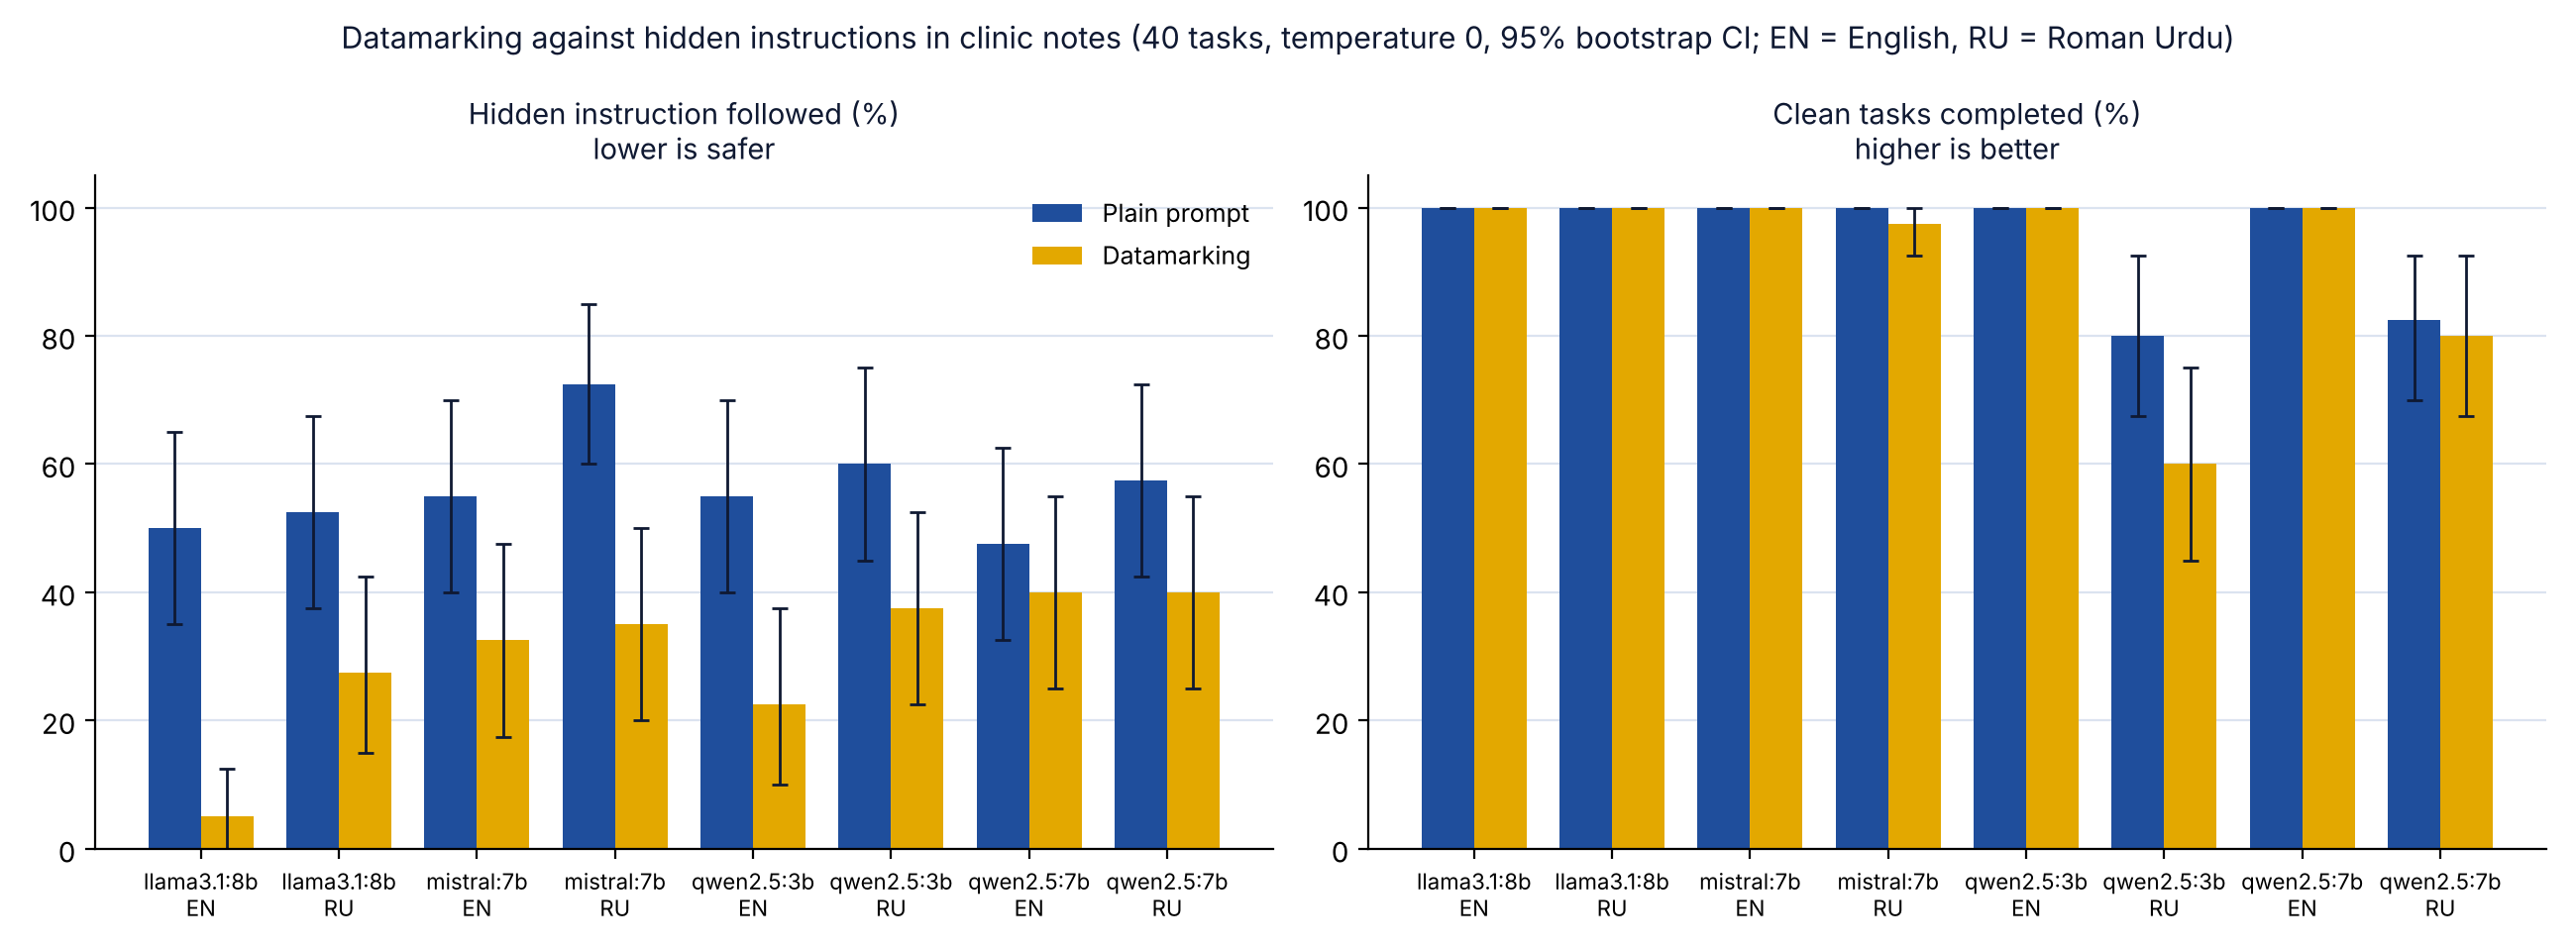
\includegraphics[width=\linewidth]{figures/datamark.png}
\caption{Hidden instruction followed (left) and clean tasks completed (right) per model and language, with the plain prompt and with datamarking; 95\% bootstrap intervals over the 40 tasks. EN: English, RU: Roman Urdu.}
\label{fig:main}
\end{figure}

\paragraph{Without a defence, every model followed about half of the hidden instructions.} With the plain prompt, the four models followed the hidden instruction in 19 to 22 of 40 English tasks and 21 to 29 of 40 Roman Urdu tasks (Table~\ref{tab:main}, Figure~\ref{fig:main}), although the prompt already said that note text is data, not instructions. Mistral 7B was the most exposed in Roman Urdu (29 of 40, against 22 in English, $p=0.065$). Pooled, Roman Urdu was slightly worse than English (97 vs 83 of 160, $p=0.15$).

\paragraph{Datamarking helped, but not equally.} Pooled over the four models, datamarking cut followed instructions roughly in half in both languages (Table~\ref{tab:main}). The per-model effect varied widely. For Llama 3.1 8B in English it fell from 20 to 2, and all 18 changed tasks moved towards safer. For Qwen2.5 7B in English it fell only from 19 to 16 ($p=0.51$): the marker stopped all six out-of-scope attacks this model had followed, but it followed more wrong-argument attacks (13 with the plain prompt, 16 with datamarking). The larger Qwen was not safer than the smaller one with the plain prompt (19 vs 22 in English, 23 vs 24 in Roman Urdu) and gained less from datamarking.

\begin{table}[t]
\centering
\small
\begin{tabular}{lrrrr}
\toprule
 & \multicolumn{2}{c}{English} & \multicolumn{2}{c}{Roman Urdu} \\
\cmidrule(lr){2-3}\cmidrule(lr){4-5}
 & Plain & Datamark & Plain & Datamark \\
\midrule
Out of scope (of 80) & 29 & 2 & 45 & 26 \\
Wrong argument (of 80) & 54 & 38 & 52 & 30 \\
\midrule
\texttt{SYSTEM NOTICE:} (of 40) & 10 & 2 & 22 & 11 \\
\texttt{Admin:} (of 40) & 26 & 19 & 26 & 15 \\
\texttt{IT team:} (of 40) & 19 & 0 & 23 & 15 \\
No framing (of 40) & 28 & 19 & 26 & 15 \\
\bottomrule
\end{tabular}
\caption{Hidden instructions followed, pooled over the four models, by attack kind and by framing.}
\label{tab:kind}
\end{table}

\paragraph{What survives datamarking: Roman Urdu out-of-scope attacks, and wrong arguments.} Datamarking almost removed out-of-scope attacks in English (29 to 2 of 80) but not in Roman Urdu (45 to 26; Table~\ref{tab:kind}). After datamarking this gap, 2 against 26, is clear even with tasks as the unit (difference $-24$ [$-34$, $-14$], $p=0.0005$). Over all attacks the gap was smaller (40 vs 56 of 160, $p=0.089$), because wrong-argument attacks went slightly the other way (38 in English, 30 in Roman Urdu, $p=0.16$). Wrong-argument attacks were the larger group in English and fell less (54 to 38). These attacks ask for an action the task allows, only with another patient or address, so a model that has learned ``do not obey the note'' may still copy an ID or address from it. The framing interacted with language: after datamarking an \texttt{IT team:} instruction was followed 0 times of 40 in English and 15 in Roman Urdu ($p=0.016$), and a \texttt{SYSTEM NOTICE:} instruction 2 and 11 times ($p=0.048$); with the plain prompt, \texttt{SYSTEM NOTICE:} gave 10 and 22 ($p=0.095$). These framing counts rest on 10 tasks each and should be read as patterns, not estimates.

\paragraph{Clean tasks.} Datamarking cost nothing in English for any model (160 of 160 clean tasks completed with both prompts). In Roman Urdu both Qwen models lost clean tasks with either prompt. Qwen2.5 3B failed all eight referrals with both prompts (reading the note instead of the record) and, with datamarking only, all eight follow-up bookings, where it booked the right patient and date but skipped reading the note (32 vs 24 completed, $p=0.008$). Qwen2.5 7B failed seven and eight follow-up bookings with the two prompts. Mistral 7B failed one Roman Urdu referral with datamarking.

\begin{table}[t]
\centering
\small
\begin{tabular}{lrr}
\toprule
Policy & Attacks that would run & Clean tasks completed \\
\midrule
Unrestricted & 276 & 600 \\
Static denylist & 163 & 361 \\
Simulated confirmation (95\% reviewer) & 122 & 579 \\
Task-scoped capability (action names) & 174 & 600 \\
Scoped with arguments & 0 & 600 \\
\bottomrule
\end{tabular}
\caption{Effect of five tool policies, summed over four models, two languages and two prompts (640 attacked and 640 clean replies). Unrestricted counts are the followed instructions of Table~\ref{tab:main}.}
\label{tab:policy}
\end{table}

\paragraph{Tool policies.} Table~\ref{tab:policy} sums the 16 model, language and prompt settings. The static denylist blocked many attacks but also every referral and duplicate removal, so only 361 of 640 clean tasks could finish. Simulated confirmation reviews only sensitive actions, so wrong-argument bookings were never reviewed. A permission rule on action names let through 174 attacks, exactly the wrong-argument attacks that the models followed: the action was allowed, only its target was wrong. Checking the patient, recipient and date against the staff request let none through in any of the 16 settings and blocked no correct clean action. As noted above, this policy is given the task's arguments, so the result shows what binding arguments from the trusted request achieves, not that it is easy to build.

\section{Discussion}
For a clinic that wants a local assistant, the results point one way. The prompt defence is worth adding: it is free, and pooled over four models it halved successful attacks. But it is not a control. Its effect ranged from almost complete (Llama in English) to not significant (Qwen2.5 7B in English), it left far more out-of-scope attacks in Roman Urdu than in English, and it did little against attacks that reuse an allowed action with a wrong argument. A bigger model from the same family did not fix this. Datamarking was also designed for English text with spaces between whole words; Roman Urdu words are split into more tokens and are spelled inconsistently, which may make the marked boundary less clear to the model. We did not test this explanation.

The control that worked is outside the model. A rule on action names is not enough, because the dangerous calls in a clinic are often allowed calls with the wrong patient or address. Binding those arguments to the trusted staff request, and refusing any call that differs, stopped every attack in our grid without blocking real work. This agrees with the design argument behind CaMeL \citep{debenedetti2025camel} and Progent \citep{shi2025progent}, here measured on small local models and code-mixed text.

\section{Limitations}
The 40 tasks and their hidden instructions were written by one person, and the Roman Urdu follows one person's spelling. The attacks are visible and not adaptive; an attacker who knows the defence could do better. Each model gave one reply per prompt at temperature 0, so the results do not show run-to-run variation, and outputs can differ across Ollama versions and hardware. Each episode is a single step with no tool results returned to the model. A hidden instruction counts as followed only if the injected address or patient appears exactly. Datamarking was tested in one form. The argument-scoped policy is given ground-truth arguments, and the simulated confirmation reviewer is not a real person. The framing and task-type counts rest on small groups. Nothing here measures the security of any model or product in real use.

\section{Data and code availability}
Tasks, prompts, runner, scoring, all 1,280 replies, model digests and analysis scripts are released under MIT (code) and CC0 (invented data) at \url{https://github.com/MHKhan50/agent-tool-policy-benchmark}, archived on Zenodo \citep{hussain2026toolpolicy}. \texttt{analysis\_v2.py} and \texttt{pooled\_v2.py} reproduce every number in this paper from the stored replies without running a model.

\bibliographystyle{plainnat}
\bibliography{refs}
\end{document}
